\chapter[Finding the magic wavelength for the birefringence protocol]{Finding the magic wavelength for the birefringence QND measurement and spin squeezing protocol for clock-state atoms trapped around a nanofiber}\label{chap:magicwavelength}
In this appendix, we provide some details on finding the magic frequency so that the photon fluctuation noise can be canceled while a QND-measurement-useful Hamiltonian can be retained. We first prove that in the case of one-frequency probe, the scalar polarizability of atoms doesn't allow a magic wavelength for our purpose; then we show that if the scalar polarizability has to be used (for example, to avoid photon scatterings among atoms), a two-color scheme may be feasible; finally, we provide some details on calculating the magic wavelength with one-color probe considering the tensor polarizability effect. We will only take the example of nanofiber, but the theory can be generalized to other nanophotonic waveguides.

Based on Chapter~\ref{chap:birefringence}, in the case that a nanofiber dispersively coupled to an atomic ensemble, the Hamiltonian per time $ \tau $ measurement can be given as below using the Stokes operators, $\hat{S}_q $, and collective spin operators, $ \hat{J}_q $, with $ q=0,1,2,3 $:
\begin{align}
H_{\rm eff} 
=\frac{\hbar}{\tau} \Big\{ & \left[ \big( \chi_{H,\uparrow} + \chi_{H,\downarrow}\big) + \big(\chi_{V,\uparrow} + \chi_{V,\downarrow}\big) \right] \hat{J}_0 \hat{S}_0 \nonumber \\
+ & \left[ \big( \chi_{H, \uparrow} + \chi_{H,\downarrow}\big) - \big( \chi_{V,\uparrow} + \chi_{V,\downarrow} \big)\right]  \hat{J}_0 \hat{S}_1 \nonumber \\
+ & \left[ \big( \chi_{H,\uparrow} - \chi_{H,\downarrow}\big) + \big(\chi_{V,\uparrow} - \chi_{V,\downarrow} \big) \right] \hat{J}_3 \hat{S}_0 \nonumber \\
+ & \left[ \big( \chi_{H,\uparrow} - \chi_{H,\downarrow}\big) - \big(\chi_{V,\uparrow} - \chi_{V,\downarrow} \big) \right]  \hat{J}_3 \hat{S}_1\Big\}.\label{eq:JScoupling}
\end{align}
If we want to estimate the state of the collective 
spins, we need to estimate the number of atoms sitting in the $ \ket{\uparrow} $ and $ \ket{\downarrow} 
$ states employing a dispersive QND measurement technique which has been well developed for the 
free-space atomic ensembles. For our system, the forth term of the Hamiltonian in 
Eq.~\eqref{eq:JScoupling} empowers us the possibility of measuring the atomic states without 
destroying them with an $ \hat{S}_3=\frac{1}{2i}(\hat{a}_H^\dagger\hat{a}_V - 
\hat{a}_V^\dagger\hat{a}_H) $ homodyne measurement. Yet, the third term of the Hamiltonian becomes 
a source of noise term that injects photon number fluctuation noise into the measurement result. 
We want to find a magic wavelength of the probe light that allows us to totally remove the third term. 
For simplicity, we call the third line of the Hamiltonian as $ \hat{H}^3_{\rm eff} $ and its coefficient before the $ \hat{J}_3\hat{S}_0 $ or the corresponding coupling strength as $ \chi_3 $. 
Similarly, we label with the number $ 4 $ for the fourth term of the Hamiltonian and its strength of coupling. 
We also denote the coupling strength in the fourth term of the Hamiltonian as $ \chi_{\rm eff} $ for the purpose of designing the measurement protocol.

As one toy model to facilitate discussions in this appendix, we suppose the probe laser is in a detuning regime below the lower frequency side of the $ D_1 $ line transition lines so that the detuning from the ground $ 6S_{1/2} $ $ \ket{f=4} $ hyperfine level to the excited $ 6P_{1/2} $ $ \ket{f'=3} $ hyperfine level is far greater than the hyperfine structure splitting of the excited states. 
We may be able to ignore the tensor component and the imaginary part of the atomic polarizability, as well as the higher level of excited states above the $ 6P_{1/2} $ energy levels. 
Baring that the vector component of the polarizability for the clock state vanishes, we only have the scalar coefficient $C_{j' f}^{(0)} =1/3  $ [see Eq.~\eqref{Eq::ScalarCoefSum}] non-zero.~\footnote{Similar case for the $ D_2 $ line, which gives $ C_{j' f}^{(0)} =2/3 $.} Therefore, the atomic polarizability tensors defined in Eq.~\eqref{eq:alphaupdown} can be given by
\begin{align}
\tensor{\boldsymbol{\alpha}}_{\uparrow} &\approx\sum_{f'=3,4}\frac{\alpha_0(\Delta_{4,f'})}{3}\unittensor \\
\tensor{\boldsymbol{\alpha}}_{\downarrow} &\approx\sum_{f'=3,4}\frac{\alpha_0(\Delta_{3,f'})}{3}\unittensor,
\end{align}
with $ \alpha_0(\Delta_{f,f'})=-\frac{3\lambda_{j'j}^3}{32\pi^3} \frac{\Gamma}{\Delta_{f,f'}} $. In our case, we can make $ \lambda_{j'j}\approx\lambda= \frac{2\pi c}{\omega_0}$. Therefore, we have
\begin{align}
\frac{2\pi\omega_0}{v_g}\alpha_0(\Delta_{f,f'})=-\frac{n_g\sigma_0}{4} \frac{\Gamma}{\Delta_{f,f'}}
\end{align}
with the 3D atomic on-resonance cross section $ \sigma_0= \frac{3\lambda^2}{2\pi}  $. 

The coupling strengths defined in Eq.~\eqref{eq:chiHVUD_2} for $ D_1 $ line probing can then be written as
\begin{align}
\chi_{H,\uparrow} &=   \frac{1}{2} \sum_{f'} \chi_{H0}(f',4) C_{j',f',4}^{(0)}  =  \frac{1}{2} \sum_{f'} \frac{\chi_{H0}(f',4)}{3} \label{chiHUp}  \\
\chi_{H,\downarrow} &=   \frac{1}{2} \sum_{f'} \chi_{H0}(f',3)  C_{j',f',3}^{(0)} = \frac{1}{2} \sum_{f'} \frac{\chi_{H0}(f',3) }{3} \label{chiHDown}\\
\chi_{V,\uparrow} &=   \frac{1}{2} \sum_{f'} \chi_{V0}(f',4)  C_{j',f',4}^{(0)}  =   \frac{1}{2} \sum_{f'} \frac{\chi_{V0}(f',4)}{3}\label{chiVUp}  \\
\chi_{V,\downarrow} &=   \frac{1}{2} \sum_{f'} \chi_{V0}(f',3)  C_{j',f',3}^{(0)}=   \frac{1}{2} \sum_{f'} \frac{\chi_{V0}(f',3) }{3} \label{chiVDown}
\end{align}
and 
\begin{align}
\chi_{H0}(f',f) &= \left( \frac{ \sigma_0}{A_{ef\!f}^H} \right) \left( \frac{\Gamma}{2 \Delta_{f,f'}} \right)\\
\chi_{V0}(f',f) &= \left( \frac{ \sigma_0}{A_{ef\!f}^V} \right) \left( \frac{\Gamma}{2 \Delta_{f,f'}} \right)\\
A_{ef\!f}^H &= \frac{1}{n_g|\mathbf{u}_{H}(r^\prime\!\!_\perp,\phi')|^2}\\
A_{ef\!f}^V &= \frac{1}{n_g | \mathbf{u}_{V}(r^\prime\!\!_\perp,\phi')|^2}.\label{eq:AeffV}
\end{align}
Considering the relations between $ \Gamma_{1D} $ and $ \Gamma_0 $ (the same as the $ \Gamma $ above, for now) from Eq.~\eqref{Gamma1DGammavac_appendix}, Eqs.~\eqref{chiHUp} and~\eqref{chiHDown} are equivalent to Eq.~\eqref{phaseshiftGamma1D} derived from the Green function method with scalar polarizability. The scalar polarizability factor of $ C_{j',f',f}^{(0)}=\frac{1}{3} $ in Eq.~\eqref{chiHUp} through Eq.~\eqref{chiVDown} indicates the possibility of transitions back into the clock states. This factor can be absorbed into the atomic scattering cross section by treating the scattering cross section as an average over all possible quantum transitions. 
Again, do not use the equations above for normal cases, since this is just a toy model to explore possible contradictories.


\section{Magic wavelength does not exist with merely scalar polarizability using a simple strategy}
First, we look at the case that the atomic polarizability tensor is reduced to a scalar, which maintain the polarization state of the light in the process of interaction. There are many ways to physically realize such an effect for atoms. 
Here, we assume the detuning of the optical field is much larger than the natural linewidth of the 
coupled atoms so that we can ignore the tensor contribution of the atomic polarizability. We have also 
restricted the atomic ground state within the $ 6S_{1/2} $ $ F=3 $ ($ \ket{\downarrow} $) and $ F=4 $ ($ 
\ket{\uparrow} $) clock state space\index{state!clock state} which rules out the vector contribution of 
the atomic polarizability. Therefore, the atomic polarizability only has a scalar polarizability effect for this problem. 

From the definition of the coupling strength of various $ \chi $'s [from Eq.~\eqref{chiHUp} to Eq.~\eqref{eq:AeffV}], one can show that, for $ D_1 $ line, 
\begin{align}
\chi_H \equiv \chi_{H,\uparrow} - \chi_{H,\downarrow} &= \frac{1}{3}\sum_{f'} \left(\frac{\sigma_0}{A_{\rm eff}^H} \right) \left(\frac{\Gamma}{4\Delta_{4f'}} - \frac{\Gamma}{4\Delta_{3f'}} \right) \nonumber\\
&= \frac{\Gamma_H}{3} \left(\frac{1}{\Delta_{43}}+\frac{1}{\Delta_{44}} - \frac{1}{\Delta_{33}}-\frac{1}{\Delta_{34}} \right) = \frac{\Gamma_H}{3}\Delta_-,\label{eq:chiH}\\
\chi_V \equiv \chi_{V,\uparrow} - \chi_{V,\downarrow} &= \frac{1}{3}\sum_{f'} \left(\frac{\sigma_0}{A_{\rm eff}^V} \right) \left(\frac{\Gamma}{4\Delta_{4f'}} - \frac{\Gamma}{4\Delta_{3f'}} \right) \nonumber\\
&= \frac{\Gamma_V}{3} \left(\frac{1}{\Delta_{43}}+\frac{1}{\Delta_{44}} - \frac{1}{\Delta_{33}}-\frac{1}{\Delta_{34}} \right)=\frac{\Gamma_V}{3}\Delta_-,\label{eq:chiV}
\end{align}
where $ \Delta_{ff'} $ is the detuning relative to the $ f\leftrightarrow f' $ transition gap, and $ \Delta_- = \left(\frac{1}{\Delta_{43}}+\frac{1}{\Delta_{44}} - \frac{1}{\Delta_{33}}-\frac{1}{\Delta_{34}} \right) $ is a common factor existing in both $ \chi_H $ and $ \chi_V $ quantities. $ \Gamma_H $ ($ \Gamma_V $) is the decay rate coupled to the forward propagating $ H $ ($ V $) mode of the nanofiber. 

To find the \emph{magic wavelength}\index{magic wavelength}, we need to make the coupling strength factor of the third term of the Hamiltonian in Eq.~\eqref{eq:JScoupling} equal to zero. That is to say,
\begin{align}
\chi_H+\chi_V=\frac{1}{3}\left(\Gamma_H + \Gamma_V \right)\Delta_- = 0.
\end{align}
We can see that $ \frac{1}{3}\left(\Gamma_H + \Gamma_V \right) $ is always positive and does not 
depending on wavelength. Therefore, we have to let $ \Delta_-=0 $ to find the "\textit{magic 
wavelength}"\index{magic wavelength}. From the definition of $ \chi_H $ and $ \chi_V $ 
(Eqs.~\eqref{eq:chiH} and~\eqref{eq:chiV}) and the Hamiltonian (Eq.~\eqref{eq:JScoupling}), we can 
find that $ \chi_H=\chi_V=0 $ and the forth term of the Hamiltonian, which is what we want to keep, also 
becomes zero. Hence, via identifying a magic wavelength and to remove the photon flux noise in the 
measurement is invalid for our initial design. Maybe we can say, the \emph{magic wavelength}\index{magic wavelength} does not 
exist for one-color probe configuration and by only considering scalar polarizability effects. 

This analytical conclusion has been numerically verified. 

\section{Calculating coupling strengths with a scalar polarizability}
Now, let us suppose we target to generating a spin squeezed state (SSS) based on the forth term of the Hamiltonian through an $ \hat{S}_3 $ homodyne QND measurement. The effective Hamiltonian becomes
\begin{align}
	H_{\rm eff} = \frac{\hbar}{\tau} \chi_{\rm eff} \hat{J}_3 \hat{S}_1
\end{align}
where $\chi_{\rm eff} = \chi_{H} - \chi_{V}=\frac{\Gamma_H-\Gamma_V}{3}\Delta_-$. As has been proved, the squeezing parameter $ \xi =\frac{\chi_{\rm eff}^2 }{4}N_LN_A $. Therefore, to calculate the squeezing parameter, we need to calculate the decay rates coupled into the $ H $ and $ V $ modes. 

Since we can treat the atomic polarizability as a scalar for our dispersive case, we have 
\begin{align}
\Gamma_H &= 2\pi \sum_g \frac{|\mathbf{u}_H(\br')\cdot \mathbf{d}_{eg}|^2}{\hbar}\left(\frac{\omega_0}{v_g} \right) \\
&\propto \sum_g \tr \left\{(\mathbf{d}_{eg}^*\mathbf{d}_{eg})\cdot \mathrm{Im} [\GFT_H^*(\br',\br')] \right\}  = \sum_f \tr \left[ \alpha_f \eye\cdot \mathrm{Im} [\GFT_H^*(\br',\br')]  \right],
\end{align}
where the atomic polarizability for the ground state $ f $ is defined as $ \alpha_f=\alpha_0(\Delta_{ff'})C_{j'f}^{(0)} $ is a scalar constant for the clock state. Using the emission surface technique introduced in Sec.~\ref{sec:geometryofemission}, the equivalent dipole momentum is pointed along $ [1,1,1]/\sqrt{3} $ direction on the principle emission coordinate system induced by the fiber $ H $-mode field. Since the $ H $ mode only has $ r\!_\perp $ and $ z $ components for an atom on the $ H $ axis, the field only couples to the corresponding $ \mathbf{e}_x $ and $ \mathbf{e}_z $ two dipole orientations with a normalization factor $ 1/3 $ for the $ D_1 $ line transitions. Similar conclusion applies to the $ \Gamma_V $ calculation yet with a $ y $ coupling. One can also consider this problem in the perspective of quantum jumps. Since all quantum transitions ($ \pi$ and $\sigma_\pm $) have the same possibility ($C_{j'ff'}^{(0)}=C_{j'f}^{(0)}=1/3 $), the decay rate is only determined by the non-zero field components with corresponding quantum transition probability. The final result does not depend on how we define the quantization axis while the details of calculation might be. 



With the knowledge of the equivalent dipole orientations, we can easily calculate the corresponding decay rates goes into the forwarding $ H $ and $ V $ modes respectively using the dipole approximation of the atom. Plots below (Figs.~\ref{fig:HVdecayrates} and~\ref{fig:squeezingparaTerms}) illustrate the decay rates and the normalized squeezing parameter $ \xi/N_LN_A $ as functions of frequency and atom positions relative to the fiber axis. $ N_L $ is the photon number counted through the photon detector during time $ \tau $ of measurement. Note that we have assumed that the decay rate is a constant within the small detuning around the D1 line transition frequency, which should be valid. Also, in Fig.~\ref{fig:squeezingparaTerms}, we made up a toy model that we assume both the third and fourth lines of the Hamiltonian alone can generate some spin squeezing with respect to $ \hat{J}_3 $ by some "technical" measurement strategies in time $ \tau $. We plot out the squeezing parameters associated with those two Hamiltonian terms in (a) and (b) of Fig.~\ref{fig:squeezingparaTerms}. If both (a) and (b) have similar values at the same frequency and atom position points, it means the coupling effect to both Hamiltonians overlap and the useful spin squeezing with the realistic Hamiltonian (in presence of both Hamiltonian terms) will be weak. If there are mismatches on the data points, in contrast, it means one can design some protocol to obtain a strong spin squeezing effect. Based on the plots, one can hardly design a good spin squeezing protocol based on the properties of the Hamiltonian. 

\begin{figure}[!tbp]
\begin{minipage}{.91\linewidth}
\centering
{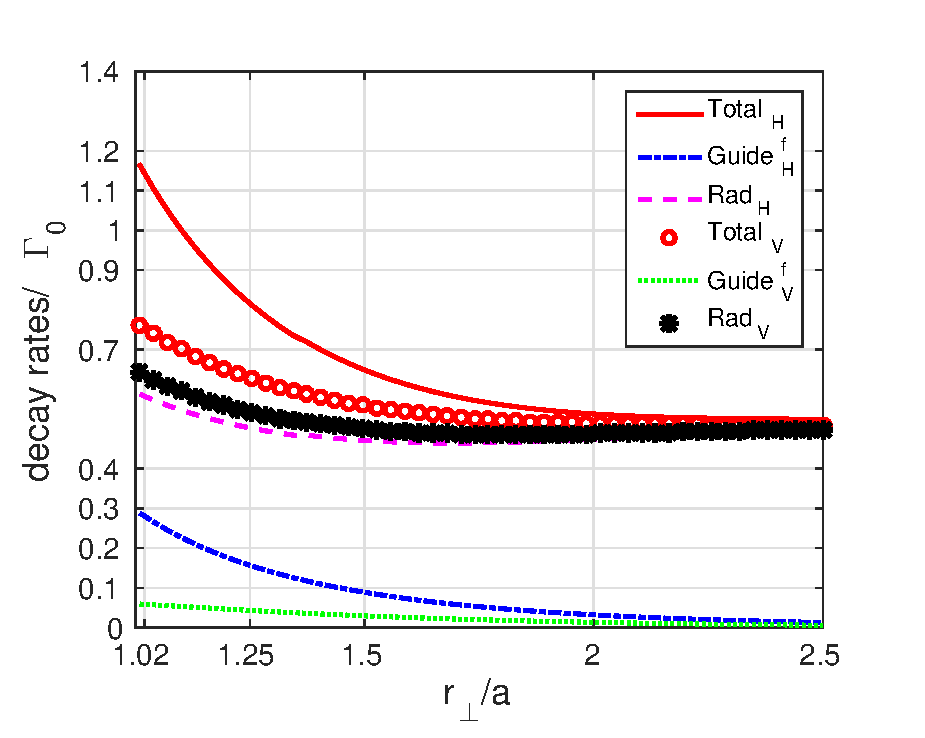
\includegraphics[scale=0.75]{../media/Figs/HVdecayrates}}
\end{minipage}
\caption[Decay rates coupled to the $ H $ and $ V $ nanofiber modes with a scalar polarizability of atoms.]{Decay rates coupled to the $ H $ and $ V $ nanofiber modes. For the guided mode contributions, only the forward propagating mode contributions are plotted out. The total decay rates for the two mode contributions have both backward and forward propagating components counted.}\label{fig:HVdecayrates}
\end{figure}

\begin{figure}[!tbp]
\begin{minipage}{.91\linewidth}
\centering
\subfloat[]{\label{squeezingparaTerm3}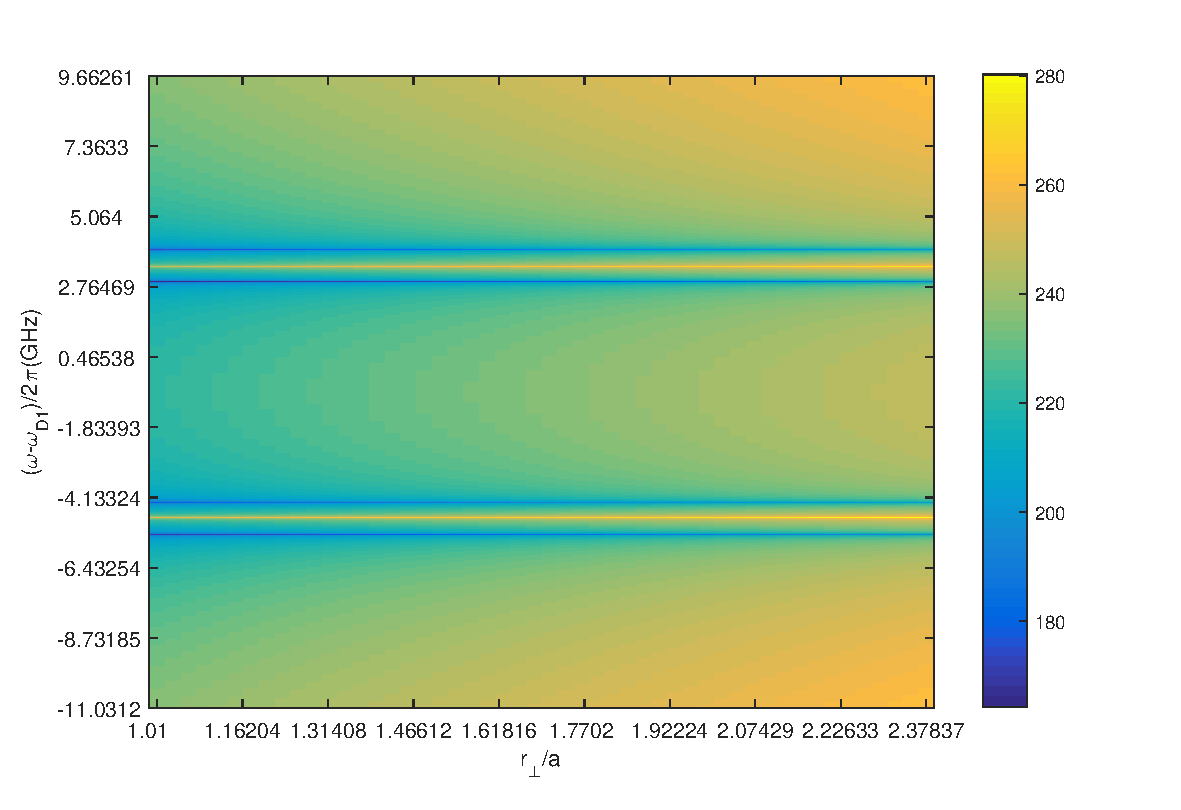
\includegraphics[scale=0.55]{../media/Figs/squeezingparaTerm3}}
\end{minipage}
\par\medskip
\begin{minipage}{.91\linewidth}
\centering
\subfloat[]{\label{squeezingparaTerm4}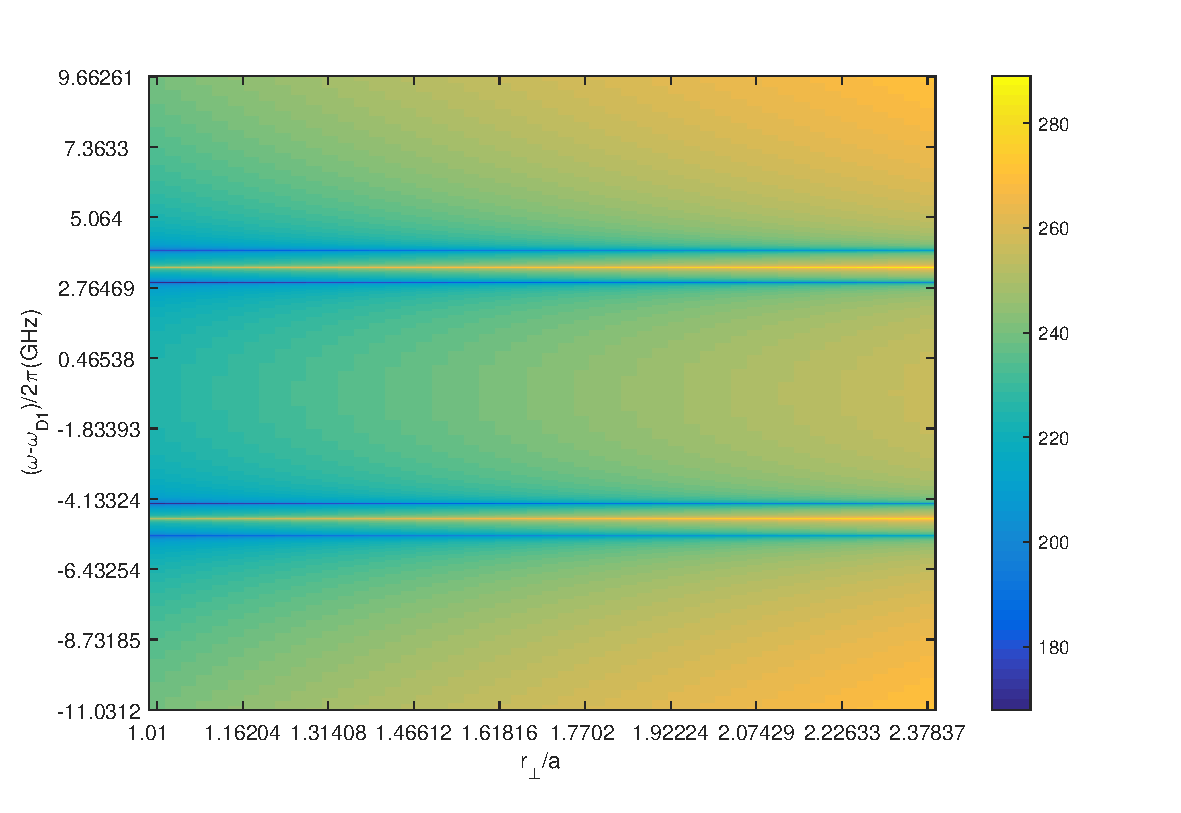
\includegraphics[scale=0.55]{../media/Figs/squeezingparaTerm4}}
\end{minipage}
\caption[Squeezing parameters as a function of frequency and the atoms' radial position using a scalar polarizability in a toy model.]{Squeezing parameters associated with the third (a) and forth (b) terms of the Hamiltonian as a function of frequency and the atoms' radial position (see text). The colormap shows the value of $ -10\log_{10}(\xi/N_LN_A) $, where $ \xi $ is the squeezing parameter and $ N_L $ is the photon number counted at the photon detector in time period $ \tau $. The calculation assumes the signal is solely generated by $ \hat{H}^3_{\rm eff} $ and $ \hat{H}^4_{\rm eff} $, respectively, which is just a toy model. We use this simulation to show the possibility of designing a good spin squeezing protocol by finding a proper frequency and some atom positions. }
\label{fig:squeezingparaTerms}
\end{figure}

\begin{figure}
\begin{minipage}{.91\linewidth}
\centering
{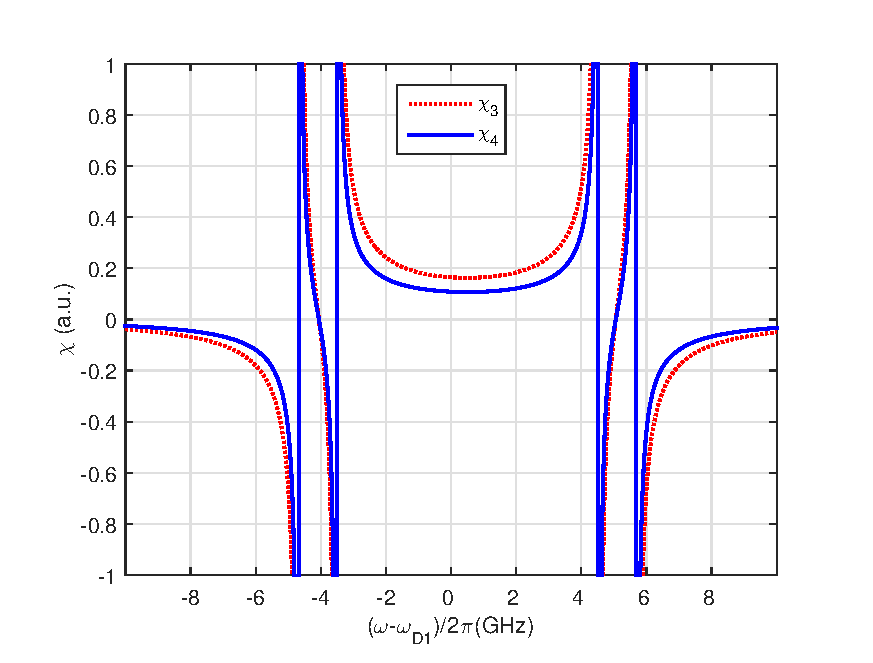
\includegraphics[scale=0.75]{../media/Figs/chi34}}
\end{minipage}
\caption[Coupling strengths as a function of detuning.]{The coupling strengths for the third ($ \chi_3 $) and forth ($ \chi_4 $) terms of the Hamiltonian expressed in Eq.~\eqref{eq:JScoupling} for the D1 line transitions associated with the clock states.} \label{fig:chi34}
\end{figure}

As shown in Fig.~\ref{fig:chi34} regarding the coupling strengths of the third and forth terms of the one-color probe Hamiltonian, the two peaks on the negative frequency side and those on the positive frequency side correspond to the approximate frequencies one can use to detect the $ \ket{\uparrow} $ and $ \ket{\downarrow} $ atom numbers. The two Hamiltonian terms seem very close to each other due to the small $ \Gamma_V $. How much the photon fluctuation affects the final result is unclear, but the noise is on the same order as the signal (projection noise).



\section{Estimate psuedo-spin state and atom number in a high resolution}
Now we come to the question "is there any way to remove the photon fluctuation from the homodyne measurement?" One way that might work is to use two-color light signals to commit the measurement. The basic idea follows. 

If we use two-color probes for each measurement configuration, it might be possible to find non-trivial magic wavelengths to cancel the third term of the Hamiltonian. The key is that, for two distinguishable colors, the decay rates coupled to the corresponding guided modes are distinguishable as well, which may result in magic wavelengths that does not totally remove the coupling strengths at the same time. For instance, if we choose the two probes around D1 and D2 transition frequencies at $ \omega_1 $ and $ \omega_2 $, the two sets of $ \Gamma_{H/V}(\omega_1) $ and $ \Gamma_{H/V}(\omega_2) $ will be different. Quantitatively, the third term of the effective Hamiltonian can now be given by
\begin{align}
\!\!\!\!\!\!\!\!\!\!\hat{H}_{\rm eff}^3(\omega_1,\omega_2) &= \frac{\hbar}{\tau} \left[\chi_H(\omega_1)+\chi_H(\omega_2) + \chi_V(\omega_1)+\chi_V(\omega_2) \right] \hat{J}_3\hat{S}_0\\
&= \frac{\hbar}{3\tau} \left[  \left( \Gamma_H(\omega_1)\!+\!\Gamma_V(\omega_1) \right)\Delta_-^1(\omega_1) \!+\! 2\left( \Gamma_H(\omega_2)\!+\!\Gamma_V(\omega_2) \right)\Delta_-^2(\omega_2) \right] ,
\end{align}
where $ \Delta_-^{1/2} $ are the detuning terms due to the two colors of the probes. Similarly, the forth term of the Hamiltonian can now be given by
\begin{align}
\!\!\!\!\!\!\!\!\!\!\hat{H}_{\rm eff}^4(\omega_1,\omega_2) &= \frac{\hbar}{\tau} \left[\chi_H(\omega_1)+\chi_H(\omega_2) - \chi_V(\omega_1)-\chi_V(\omega_2) \right] \hat{J}_3\hat{S}_0\\
&= \frac{\hbar}{3\tau} \left[  \left( \Gamma_H(\omega_1)\!-\!\Gamma_V(\omega_1) \right)\Delta_-^1(\omega_1) \!+\! 2\left( \Gamma_H(\omega_2)\!-\!\Gamma_V(\omega_2) \right)\Delta_-^2(\omega_2) \right] .
\end{align}
Now that, the magic wavelengths canceling the third term of the Hamiltonian may not result in a zero coupling strength for the forth term of the Hamiltonian due to the inseparability of decay rates and detuning factors. A two-color scheme has been tested in experiments by the QUANTOP group in Denmark for QND measurement~\cite{Beguin2014}, but it's more about using the differential phase shifts between the two probes to magnify the signal-to-noise ratio than using an precise magic wavelength to cancel the noise sources. 


\section{Magic wavelength exists by including tensor polarizability effect}
Finally, if we include the tensor polarizability effect into the Hamiltonian, and use the $ x $-axis as the 
quantization axis, the Hamiltonian can still be given in the form of Eq.~\ref{eq:JScoupling} yet with a 
tensor-response definition of the coupling strengths:
\begin{align}
\chi_{H,\uparrow/\downarrow} & \equiv \chi_{H,f} =- \frac{2\pi \omega_0}{v_g} \bra{f,0} 
	\mathbf{u}^*_H(r^\prime\!_\perp, \phi') \cdot \tensor{\alpha} \cdot 
	\mathbf{u}_{H}(r^\prime\!_\perp, 
	\phi') \ket{f,0} \\
	& =- \frac{2\pi \omega_0}{v_g} \sum_{f'} \sum_q \alpha_0\left( f,f'  \right) |\mathbf{e}_q \cdot 
	\mathbf{u}_H^*(r^\prime\!_\perp,\phi')|^2 |o^{j'f'}_{jf} |^2 
	|C^{f 0;1q}_{f' q}|^2\\
	& \approx  \frac{1}{2} \left( \sigma_0 n_g  \right) \sum_{f'} \sum_q\left( 
		\frac{\Gamma}{2 
		\left(\Delta_{f,f'}+i\Gamma/2\right) }  \right)\nonumber\\
		&\quad\quad\quad\quad\quad\quad\quad\quad\quad \times |\mathbf{e}_q \cdot 
		\mathbf{u}_H^*(r^\prime\!_\perp,\phi')|^2 |o^{j'f'}_{jf} |^2 
		|C^{f 0;1q}_{f' q}|^2,\\
\chi_{V,\uparrow/\downarrow} & \equiv \chi_{V,f} =- \frac{2\pi \omega_0}{v_g} \bra{f,0} 
	\mathbf{u}^*_V(r^\prime\!_\perp, \phi') \cdot \tensor{\alpha} \cdot 
	\mathbf{u}_{V}(r^\prime\!_\perp, 
	\phi') \ket{f,0} \\
	& =- \frac{2\pi \omega_0}{v_g} \sum_{f'} \sum_q \alpha_0\left( f,f'  \right) |\mathbf{e}_q \cdot 
	\mathbf{u}_V^*(r^\prime\!_\perp,\phi')|^2 |o^{j'f'}_{jf} |^2 
	|C^{f 0;1q}_{f' q}|^2\\
	& \approx  \frac{1}{2} \left( \sigma_0 n_g  \right) \sum_{f'} \sum_q\left( 
		\frac{\Gamma}{2 
		\left(\Delta_{f,f'}+i\Gamma/2\right) }  \right)\nonumber\\
		&\quad\quad\quad\quad\quad\quad\quad\quad\quad \times |\mathbf{e}_q \cdot 
		\mathbf{u}_V^*(r^\prime\!_\perp,\phi')|^2 |o^{j'f'}_{jf} |^2 
		|C^{f 0;1q}_{f' q}|^2,
\end{align}
where we have approximated $ \lambda_{j'}\approx \lambda = \frac{2\pi c}{\omega_0} $.  

The magic wavelengths/frequencies using the one-probe configuration can be found close to the $ 
f=3\rightarrow f'=3 $ and $ f=4\rightarrow f'=4 $ two transitions.
The spin squeezing parameters solely due to $ \hat{H}^3_{\rm eff} $ and $ \hat{H}^4_{\rm eff} $ can be calculated for our toy model as has been discussed earlier.
Plots for the coupling strengths and magic frequencies can be found in 
Figs.~\ref{fig:MagicwavelengSqueezingpara},~\ref{fig:squeezingparaTerms_total} 
and~\ref{fig:chi34_total}.

\begin{figure}[!tbp]
\begin{minipage}{.91\linewidth}
\centering
\subfloat[]{\label{MagicwavelengSqueezingpara1}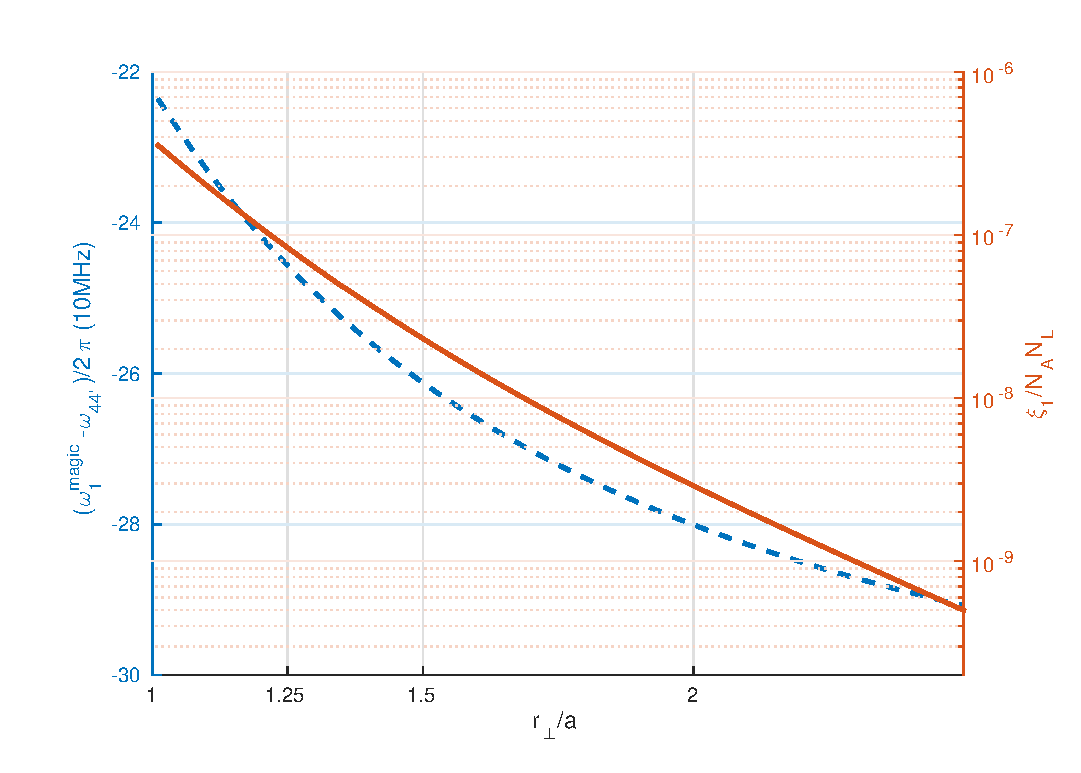
\includegraphics[scale=0.65]{../media/Figs/MagicwavelengSqueezingpara1}}
\end{minipage}
\par\medskip
\begin{minipage}{.91\linewidth}
\centering
\subfloat[]{\label{MagicwavelengSqueezingpara2}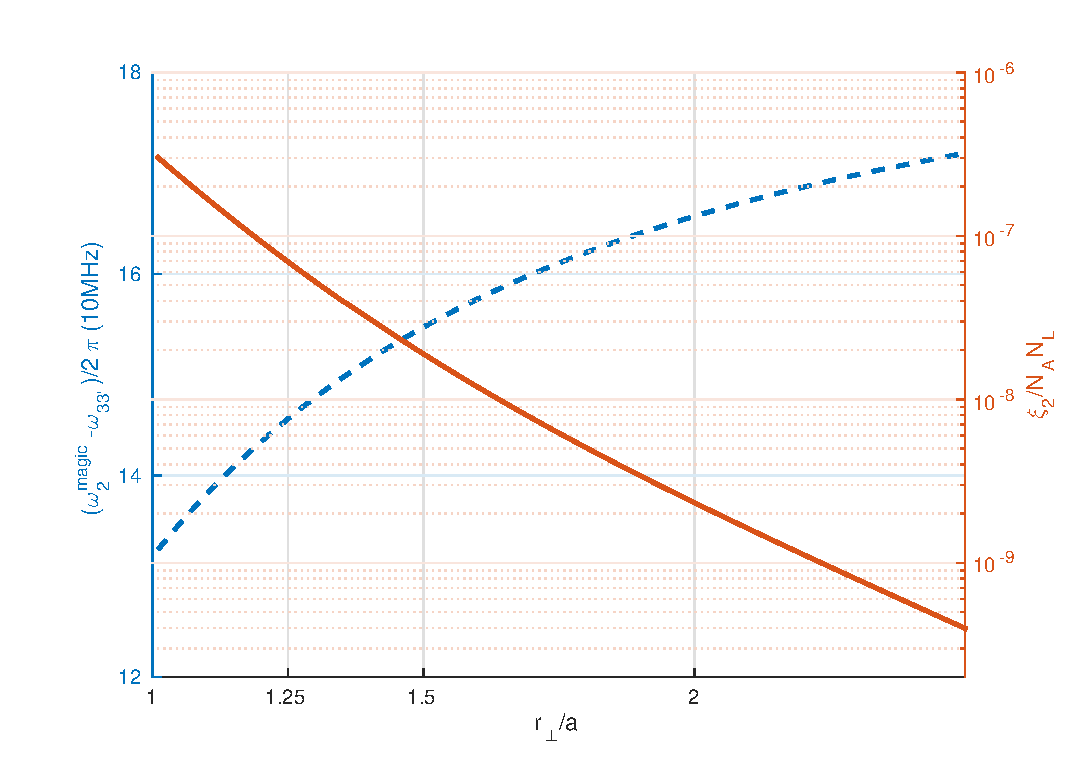
\includegraphics[scale=0.65]{../media/Figs/MagicwavelengSqueezingpara2}}
\end{minipage}
\caption[Magic frequencies and spin squeezing including the tensor interactions.]{The magic frequencies (left axis and dashed lines) and corresponding squeezing parameters 
(right axis and solid lines) close to the $ 
f=3\rightarrow f'=3 $ (b) and $ f=4\rightarrow f'=4 $ (a) transition lines. The squeezing parameters are 
normalized for per photon per atom squeezing. }\label{fig:MagicwavelengSqueezingpara}
\end{figure}

\begin{figure}[!tbp]
\begin{minipage}{.91\linewidth}
\centering
\subfloat[]{\label{squeezingparaTerm3_total}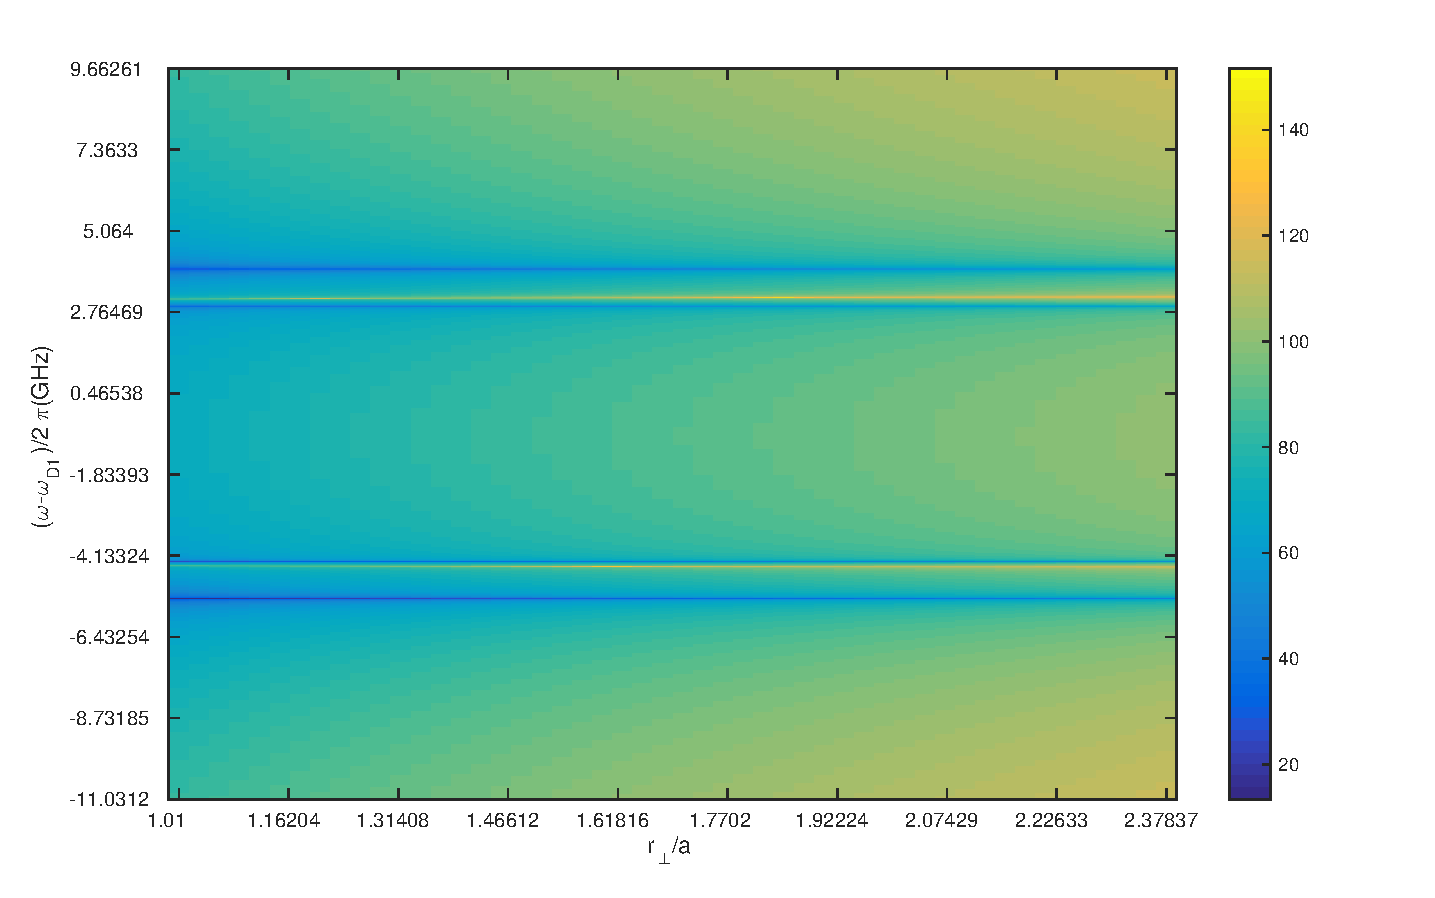
\includegraphics[scale=0.55]{../media/Figs/squeezingparaTerm3_total}}
\end{minipage}
\par\medskip
\begin{minipage}{.91\linewidth}
\centering
\subfloat[]{\label{squeezingparaTerm4_total}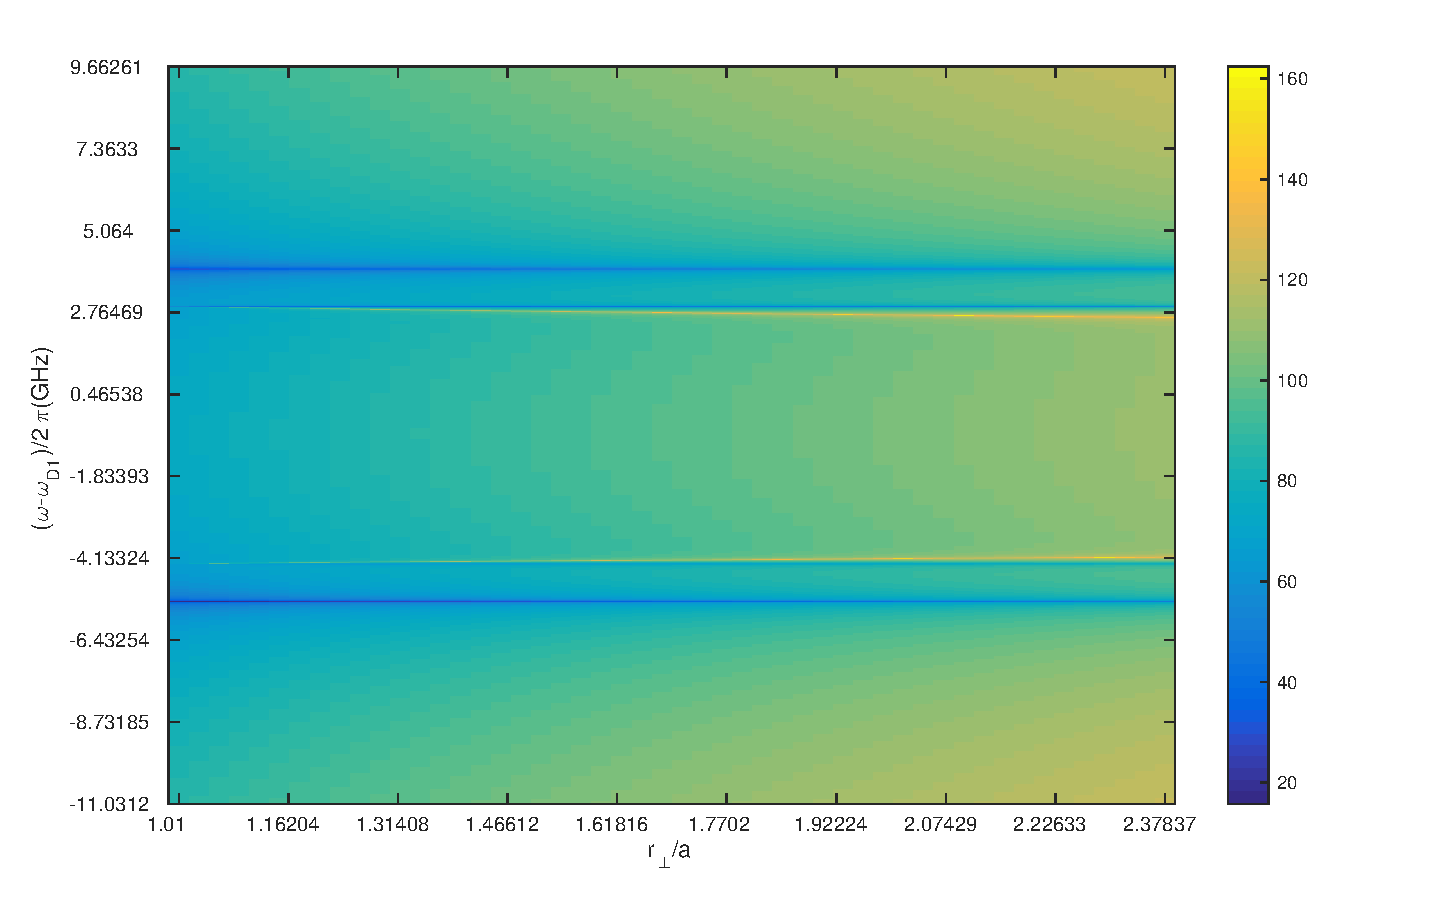
\includegraphics[scale=0.55]{../media/Figs/squeezingparaTerm4_total}}
\end{minipage}
\caption[Squeezing parameters as a function of detuning and atom position with a full atomic polarizability.]{Similar to Fig.~\ref{fig:squeezingparaTerms}, squeezing parameters associated with the third (a) and forth (b) terms of the Hamiltonian in a toy model. The 
colormap shows the value of $ -10\log_{10}(\xi/N_LN_A) $.  All atomic polarizability components are included. We see there are some pattern-mismatch areas to design a good spin squeezing protocol to cancel the noise sources while still retain a strong useful coupling Hamiltonian.}
\label{fig:squeezingparaTerms_total}
\end{figure}

\begin{figure}[!tbp]
\begin{minipage}{.91\linewidth}
\centering
{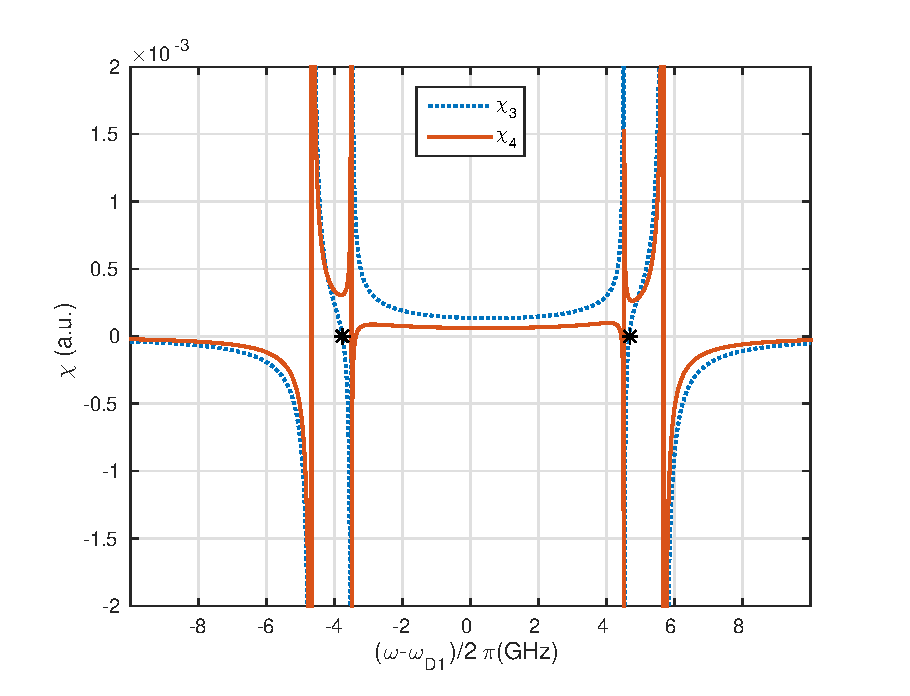
\includegraphics[scale=0.75]{../media/Figs/chi34_total}}
\end{minipage}
\caption[The coupling strengths in the birefringence-interaction Hamiltonian 
calculated for the D1 line transitions associated with the clock states to find the magic frequencies.]{The coupling strengths, $ \chi_3 $ and $ \chi_4 $, in the Hamiltonian 
expressed in Eq.~\eqref{eq:JScoupling} calculated for the D1 line transitions associated with the clock states.
All atomic polarizability components are included. The stars indicate where the magic frequencies are existed. The value of $ \chi_4 $ is considerable at the two magic frequencies.}  
\label{fig:chi34_total}
\end{figure}
